%        File: README.tex
%     Created: 一 12月 30 04:00 下午 2019 C
% Last Change: 一 12月 30 04:00 下午 2019 C
%
\documentclass{ctexart}
\usepackage[a4paper,left=2.0cm,right=2.0cm,top=2.0cm,bottom=2.0cm]{geometry}
\usepackage{graphicx}
\usepackage{fancyhdr}
\usepackage{amsmath}
\usepackage{amssymb}
\usepackage{xeCJK}
\usepackage{listings}
\usepackage{float}
\CTEXsetup[format={\Large\bfseries}]{section}
\usepackage{xcolor}
\lstset{language = c,numbers=left, showstringspaces=false, keywordstyle= \color{ blue!70 },commentstyle=\color{red!50!green!50!blue!50}, frame=shadowbox, rulesepcolor= \color{ red!20!green!20!blue!20 } 
} 
\cfoot{\thepage}
\title{分布式上机作业}


\author{}
\date{}
\begin{document}
\maketitle
\zihao{5}
\CJKfamily{zhsong}


\section{小组成员}
%\begin{center}
  \begin{tabular}{lc}
	冯吕 & $201928013229158$\\
	刘丁玮 & $2019E8013261029$\\
	孙佳钰 & $2019E8013261049$\\
	解伟凡 & $201928013229128$
\end{tabular}
%\end{center}

\section{快照算法}
\begin{itemize}
  \item  源程序:$snapshot/snapshot.c$
  \item 编译运行:$./snapshot/brun.sh$
	\item 说明:两个进程$p$和$q$通过两个通道轮转消息$message$,当进程$p$状态为$101$,即收到消息101次,之后把消息再次发送出去,然后开始快照算法,算法会记录两个进程的状态和通道状态。
\end{itemize}

\section{锁服务}
\begin{itemize}
  \item 锁服务实现代码:$LockService/include, LockService/src$
  \item 编译:$./LockService/build.sh\ r$
\end{itemize}

\subsection{API}
\subsubsection{锁服务器}
\begin{lstlisting}
#include <iostream>

#include <LockServer.h>

int main()
{
    LockServer ls(8080, 5);
    ls.init();
    ls.run();
}
\end{lstlisting}
锁服务器的创建非常简单。例如,上面的代码创建了一个锁服务器$ls$,第一个参数为服务器监听的端口号,第二个参数为可选参数,设置服务器的工作线程数目为5,默认值为$2$;$ls.init()$进行服务器初始化工作;$ls.run()$开始运行服务器。

\subsubsection{锁客户端}
\begin{lstlisting}
#include <iostream>
#include <string>
#include <thread>

#include "LockClient.h"

int share_number = 0;
LockID lock_id = 1;
void worker(PID pid)
{
    LockClient lc("localhost", 8080);
    Status s;
    for (size_t i = 0; i < 10; ++i)
    {
        s = lc.acquire(lock_id, pid);

        std::cout << "Pid = " << pid << ", "
                  << "share_number = " << share_number << std::endl;
        ++share_number;

        s = lc.release(lock_id, pid);
    }
}


int main()
{
    std::thread t1(worker, 1);
    std::thread t2(worker, 2);
    std::thread t3(worker, 3);
    t1.join();
    t2.join();
    t3.join();
    std::cout << "The final value of share_number is " 
              << share_number << std::endl;
    return 0;
}
\end{lstlisting}
锁客户端的创建同样非常简单,如上述第$11$行代码所示,创建client时需要指定服务器的$ip$地址和端口号,上面的代码指定服务器为本地服务器,端口号为$8080$。Client 提供两个方法:$acquire$和$release$。
\begin{itemize}
  \item $acquire$:申请锁,参数为锁$id$和进程$id$;
	\item $release$:释放锁,参数同样为锁$id$和进程$id$。
\end{itemize}
上述代码为三个线程通过锁服务互斥访问一个共享变量,每次访问将共享变量的值加一。上述程序运行的结果如下图所示:
\begin{figure}[H]
  \centering
  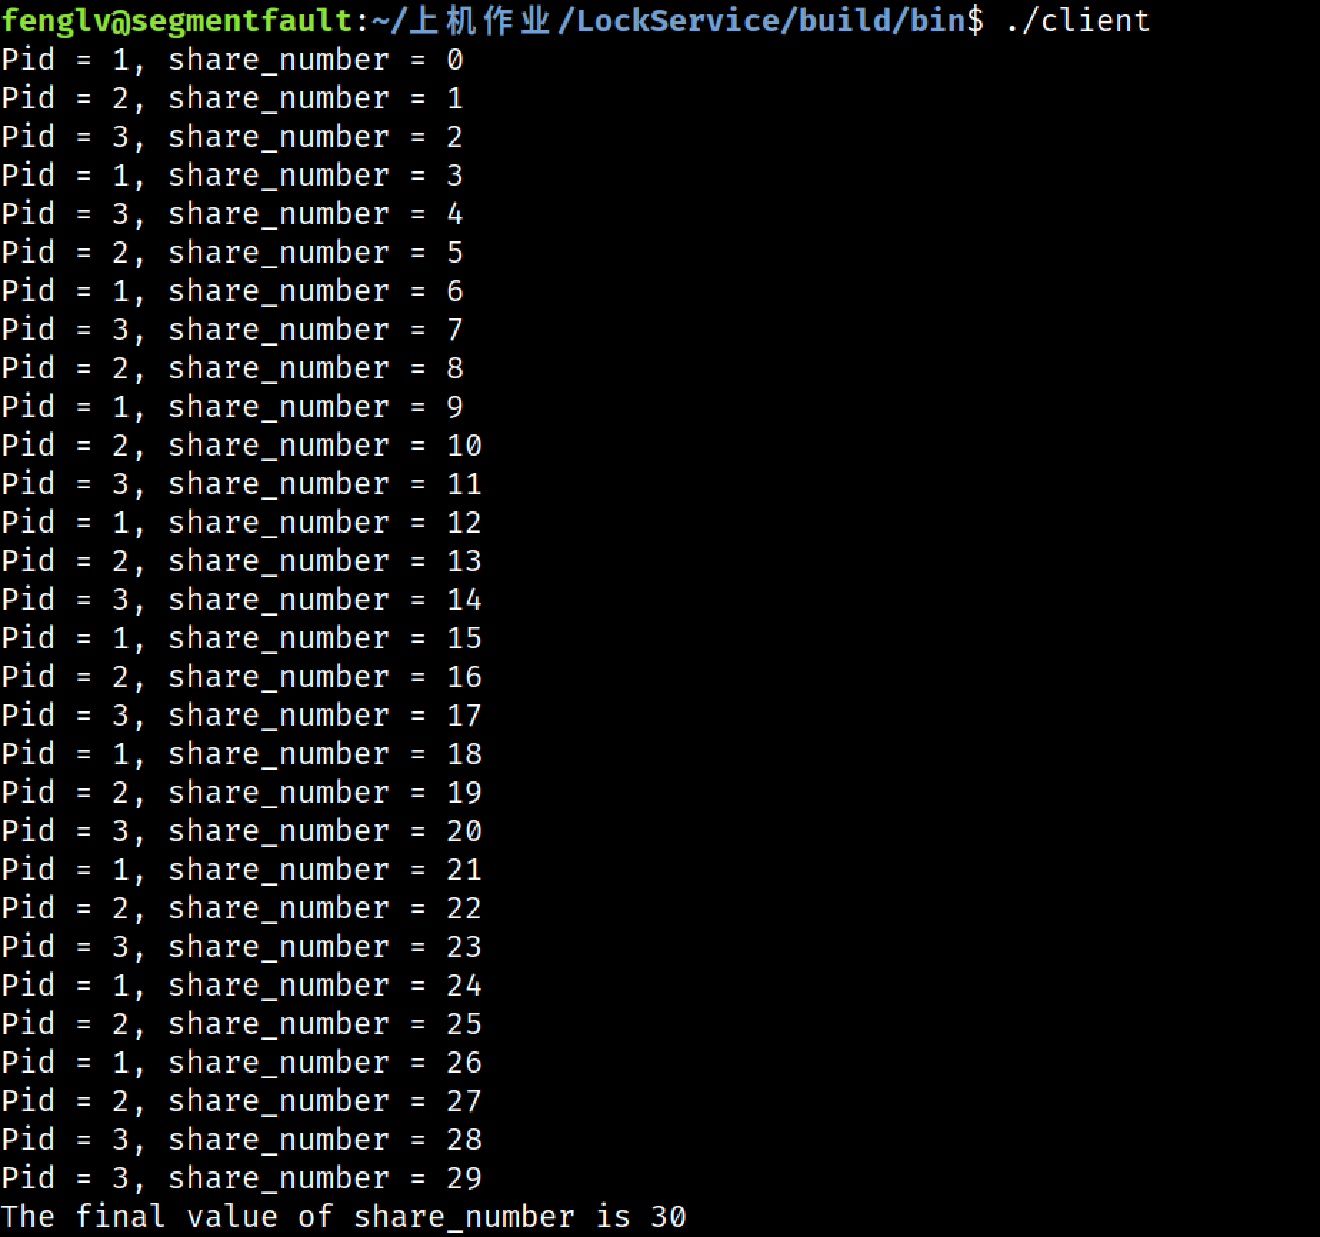
\includegraphics[width = \textwidth]{./client.pdf}
\end{figure}

\end{document}



